\documentclass[12pt, letterpaper]{article}

%-------Packages---------
\usepackage{newpxtext,newpxmath} % Palatino-like text & math (modern)
\usepackage{bboldx}
\usepackage{mathtools}
\usepackage{tikz}
\usetikzlibrary{calc,intersections}
\usepackage{tikz-cd}
\usepackage[all,arc]{xy}
\usepackage{graphicx}

\usepackage{enumerate}
\usepackage[dvipsnames]{xcolor}
\usepackage{float}
\usepackage[left=1in,top=1in,right=1in,bottom=1in]{geometry}
\usepackage[nocheck]{fancyhdr}
\usepackage{multicol}
\usepackage{setspace}

\usepackage{dsfont}
\usepackage{mathrsfs}

\usepackage{tcolorbox}
\tcbuselibrary{theorems,skins,breakable}

\usepackage{xparse}
\usepackage{import}
\usepackage[utf8]{inputenc}

\usepackage{hyperref}
\usepackage{cleveref}
\usepackage{mdframed}

\usepackage{xcolor, ifthen, tcolorbox}
\tcbuselibrary{theorems,skins,breakable}
% Theorem System
% The following environments are provided:
%   New Problem:        \begin{problem} ...
%   New Question Header:   \qh (then followed by subproblems)
%   Subproblem:     \begin{subproblem} ...
%   Problem Proof:  \begin{problemproof} ...
%   Proof:          \\begin{pf}{color} ...
%   Remark:         \rmk (sentence), \rmkb (block)

% Define custom colors
\definecolor{thmscol}{HTML}{F4565B} %For Problems
\definecolor{lemscol}{HTML}{FE844C} %For Lemmes
\definecolor{prpscol}{HTML}{00A7EF} %For proposition
\definecolor{corscol}{HTML}{23DAFF} %For corrolaries
\definecolor{rmkscol}{HTML}{6DEEC5} %For remarks
\definecolor{defscol}{HTML}{18C991} %For definitions
\definecolor{exmscol}{HTML}{7DB800} %For examples
\definecolor{clmscol}{HTML}{165c58} %For claims

%Change between dark(black)/light(white) mode
\newcommand{\colormode}{white}
\ifthenelse{\equal{\colormode}{white}}
      {\newcommand{\TextColor}{black}}
      {\newcommand{\TextColor}{white}}
\newcommand{\pbcolormain}{thmscol!80!\colormode}
\newcommand{\pbcolorsecond}{thmscol!38!\colormode}


% ============================
% Problem Counter
% ============================
\newcounter{subproblemcounter}
\newcounter{problemcounter}

\newcommand{\q}{
    \setcounter{subproblemcounter}{0}%
    \stepcounter{problemcounter} % Increment problem counter
    \color{\TextColor}Problem \arabic{problemcounter}: % Display the problem counter
}

\newcommand{\stepsub}{
    \stepcounter{subproblemcounter}%
    \color{\TextColor}(\alph{subproblemcounter})
}
% ============================
% Problem
% ============================
\newtcolorbox{pb}[1]{
  enhanced,
  frame hidden,
  titlerule=0mm,
  toptitle=1mm,
  bottomtitle=1mm,
  fonttitle=\bfseries\large,
  coltitle=black,
  colbacktitle=\pbcolormain,
  colback=\pbcolorsecond,
  title={\q #1},
  coltext=\TextColor
}

\newtcolorbox{spb}[1]{
  enhanced,
  frame hidden,
  titlerule=0mm,
  toptitle=1mm,
  bottomtitle=1mm,
  fonttitle=\bfseries\large,
  coltitle=black,
  colbacktitle=\pbcolormain,
  colback=\pbcolorsecond,
  title={\stepsub #1},
  coltext=\TextColor,
  attach boxed title to top left={xshift=3mm,yshift=-2mm},
  boxed title style={
    colback=\pbcolormain,
    colframe=\pbcolormain,
  }
}

\newtcolorbox{pbh}[1]{
    enhanced,
    frame hidden,
    titlerule=0mm,
    toptitle=1mm,
    bottomtitle=1mm,
    fonttitle=\bfseries\large,
    coltitle=black,
    colbacktitle=\pbcolormain,
    colback=\pbcolorsecond,
    title={\q #1},
    boxrule=0pt,
    interior hidden,
    attach boxed title to top left={xshift=3mm,yshift=-2mm},
    boxed title style={
        colback=\pbcolormain,
        colframe=\pbcolormain,
    }
}

\newenvironment{problem}[1]{%
  \newpage
  \begin{pb}{#1}
    }{
  \end{pb}
}

\newenvironment{subproblem}[1]{%
  \begin{spb}{#1}
    }{
  \end{spb}
}

\newenvironment{problemproof}{%
    \begin{pf}{\pbcolormain}
        }{
    \end{pf}
}

\newcommand{\qh}[1][]{
    \newpage
    \begin{pbh}{#1}\end{pbh} % Display the problem counter
}

% ============================
% Claim
% ============================

\newtcbtheorem[number within=problemcounter]{claim}{Claim}
{
    enhanced,
    frame hidden,
    titlerule=0mm,
    toptitle=1mm,
    bottomtitle=1mm,
    fonttitle=\bfseries\large,
    coltitle=black,
    colbacktitle=clmscol!50!\colormode,
    colback=clmscol!20!\colormode,
}{clm}

\NewDocumentCommand{\clm}{m+m}{
    \begin{claim*}{#1}{}
        #2
    \end{claim*}
}

\newenvironment{clmpf}{
	{\noindent{\it \textbf{Proof.}}
	\setlength{\parindent}{0pt}
	}
	\tcolorbox[blanker,breakable,left=5mm,parbox=false,
    before upper={\parindent15pt},
    after skip=10pt,
	borderline west={1mm}{0pt}{clmscol!50!\colormode}]
}{
    \textcolor{clmscol!50!\colormode}{\hbox{}\nobreak\hfill$\blacksquare$}
    \endtcolorbox
}

\NewDocumentCommand{\clmp}{m+m+m}{
    \begin{claim*}{#1}{}
        #2
    \end{claim*}

    \begin{clmpf}
        #3
    \end{clmpf}
}


% ============================
% Proof
% ============================

\newenvironment{pf}[1]{%
  \def\pfcolor{#1}% Store the color in a macro
  \noindent{\it \textbf{Proof.}}%
  \tcolorbox[blanker,breakable,left=5mm,parbox=false,%
    before upper={\parindent15pt},%
    after skip=10pt,%
    borderline west={1mm}{0pt}{\pfcolor},%
    coltext=\TextColor
  ]%
  \setlength{\parindent}{0pt}%
}{%
  \textcolor{\pfcolor}{\hbox{}\nobreak\hfill$\blacksquare$}%
  \endtcolorbox%
}

\newtcolorbox{solution}{
  blanker,
  breakable,
  left=5mm,
  parbox=false,%
  before upper={\parindent15pt},%
  after skip=10pt,%
  borderline west={1mm}{0pt}{\pbcolormain},%
  coltext=\TextColor
}


% ============================
% Remark
% ============================


\NewDocumentCommand{\rmk}{+m}{
    {\it \color{rmkscol!100!white}#1}
}

\newenvironment{remark}{
    \par
    \vspace{5pt}
    \begin{minipage}{\textwidth}
        {\par\noindent{\textbf{Remark.}}}
        \tcolorbox[blanker,breakable,left=5mm,
        before skip=10pt,after skip=10pt,
        borderline west={1mm}{0pt}{rmkscol!80!\colormode},
        coltext=\TextColor
        ]
}{
        \endtcolorbox
    \end{minipage}
    \vspace{5pt}
}

\NewDocumentCommand{\rmkb}{+m}{
    \begin{remark}
        #1
    \end{remark}
}


% Define a new command for problems
\renewcommand{\headrule}{\color{\TextColor}\hrulefill}
\newcommand{\C}{\mathbb{C}}
\newcommand{\R}{\mathbb{R}}
\newcommand{\Q}{\mathbb{Q}}
\newcommand{\Z}{\mathbb{Z}}
\newcommand{\N}{\mathbb{N}}
\renewcommand{\P}{\mathbb{P}}
\newcommand{\F}{\mathbb{F}}
\newcommand{\contr}{\Rightarrow \Leftarrow}
\newcommand{\s}{\(\,\)}
\renewcommand{\t}[1]{\text{#1}}

\newcommand{\skcgen}{{\sf Gen}} 
\newcommand{\skcenc}{{\sf Enc}}
\newcommand{\skcdec}{{\sf Dec}}
\newcommand{\mac}{{\sf MAC}}
\newcommand{\ver}{{\sf Vrfy}}
\newcommand{\bit}{{\{0,1\}}}
\newcommand{\from}{\leftarrow}
\newcommand{\com}{\mathrm{com}}
\newcommand{\sample}{\overset{\$}{\leftarrow}}

% Meta data
\setstretch{1.2}

\begin{document}
\color{\TextColor}
\pagecolor{\colormode}
\setlength{\parindent}{0pt}
\pagestyle{fancy}
\fancyhf{}
\fancyhead[LOE]{\color{\TextColor}\slshape{\textbf{Vincent Ferrara}}}
\fancyhead[ROE]{\color{\TextColor}HW4 --- \thepage}
\fancyhead[C]{\color{\TextColor}EECS 475}


\begin{problem}{}
    Prove that any public key encryption (even randomized) cannot be perfectly secure. 
\end{problem}
\begin{problemproof}
    Let $(\skcgen, \skcenc, \skcdec)$ be a public key encryption on $n$ bits.
    
    Let $m_0,m_1$ be distinct messages.

    Consider the adversary $A$ s.t. we first send $m_0,m_1$ and the challenger will send back either $c=\skcenc(m_i,p_k)$ for $i \in \bit$.
    \begin{itemize}
        \item Input $(c,p_k)$
        \begin{itemize}
            \item For each $r \in$ the secret key space
            \begin{itemize}
                \item Check if $\skcdec(r,c) = m_0$
                \item If yes return 0
            \end{itemize}
        \end{itemize}
        \item return 1
    \end{itemize}
    Since we can check every key this implies that assuming the scheme is correct then we will return 0 if the $i=0$ with non-negligible probability since $\skcdec(r,c)=m_0$ with non-negligible probability given $r$ is the secret key, and
    we will return 0 if $i=0$ with negligible probability.

    Thus, $\P[i = 0 \mid A(p_k,c)=0] \neq \P[i=0 \mid A(p_k,c)=1]$.

    But perfect secrecy requires $\P[i=0 \mid C =c] = \P[i=0] = 1/2$ given $m_i$ is picked uniformly.

    This implies it will also be independent of any function on the cipher text.

    Thus, $\P[i=0 \mid A = a] = \P[i=0]$ for $a \in \bit$. However, since $\P[i = 0 \mid A(p_k,c)=0] \neq \P[i=0 \mid A(p_k,c)=1]$ this implies $\P[i=0 \mid A=a] \neq \P[i=0]$.

    Thus, this shows that there exists an algorithm for all public key encryption schemes that can give us more information.
\end{problemproof}

\begin{problem}{}
    Alice and Bob
want to securely compute the following circuit using a garbled circuit scheme.
In the following circuit, 
The input wires marked $A$ and $C$ are Alice's input,
and the input wires 
marked $B$ and $D$ are Bob's input.
Alice will act as the garbler, and Bob will act as the evaluator.

\begin{figure}[H]
        \centering
        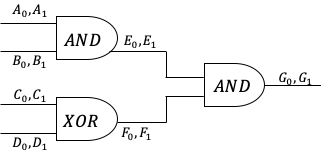
\includegraphics[scale = 0.6]{garbled.png}
        \caption{The circuit and the garbled labels on each wire.}
        \label{fig:insert}
\end{figure}

Alice does not want to make computational assumptions. 
Therefore, she  
decides to encrypt the truth table for each gate using a variant of one-time pad instead. 
Specifically for the circuit above, she randomly picks label for each wire as follows:
\begin{itemize}
    \item $G_0, G_1\leftarrow\{0,1\}^n$.
    \item $E_b,F_b\leftarrow\{0,1\}^{2n}$ for $b\in\{0,1\}$.
    \item $A_b, B_b, C_b, D_b\leftarrow\{0,1\}^{3n}$ for $b\in\{0,1\}$.
\end{itemize}

Then to encrypt each entry in the truth table, Alice uses the following scheme.
\begin{itemize}
    \item $\skcenc_{k,k'}(m):$ output $c = k\oplus k'\oplus(0^n\|m)$.
    \item $\skcdec_{k,k'}(c):$ compute $m_0\|m_1 = c\oplus k\oplus k'$ where $m_0=|n|$. If $m_0 = 0^n$, output $m_1$; otherwise, output $\bot$.
\end{itemize}
For example, for the first AND gate, Alice computes 
\begin{center}
    \begin{tabular}{|c|} 
    \hline
    $\skcenc_{A_0,B_1}(E_0)$\\
    \hline
    $\skcenc_{A_1,B_0}(E_0)$\\
    \hline
    $\skcenc_{A_0,B_0}(E_0)$\\
    \hline
    $\skcenc_{A_1,B_1}(E_1)$\\
    \hline
    \end{tabular}
\end{center}


Unfortunately, this encryption makes the garbled circuit insecure and leaks additional information beyond the inherent leakage (i.e., what is already leaked by the output). 
In this question, you are asked to  
show that Bob can break the security of the scheme step by step guided
by our hints. 

Suppose Bob's input is $0$ to wire $B$ and $1$ to wire $D$. We do not know Alice's input to wire $A$ and to wire $C$. Note that Bob only gets the garbled circuit, garbled input, and the output wire labels.
\end{problem}

\begin{subproblem}{}
    Describe how Bob can compute both $E_0$ and $E_1$ given the garbled truth tables.
\end{subproblem}
\begin{problemproof}
    For the first AND gate the garbled table entries are

    \[
    \begin{array}{c}
    c_{01} = \text{Enc}_{A_0,B_1}(E_0) = A_0 \oplus B_1 \oplus (0^n || E_0)\\
    c_{10} = \text{Enc}_{A_1,B_0}(E_0) = A_1 \oplus B_0 \oplus (0^n || E_0)\\
    c_{00} = \text{Enc}_{A_0,B_0}(E_0) = A_0 \oplus B_0 \oplus (0^n || E_0)\\
    c_{11} = \text{Enc}_{A_1,B_1}(E_1) = A_1 \oplus B_1 \oplus (0^n || E_1)
    \end{array}
    \]

    Bob's real input on this gate is \(B=0\), so he receives the label \(B_0\).
    He also gets one of \(A_0\) or \(A_1\) depending on Alice's bit \(A\).

    He tries to decrypt each row with his two labels \((A_b,B_0)\).
    Exactly one row will give something of the form \(0^n||m\) since the rest will give ; that row contains \(E_0\).

    So from some ciphertext \(c_{b0}\) he computes

    \[
    \text{Dec}_{A_b,B_0}(c_{b0}) = 0^n || E_0
    \]
    and hence learns \(E_0\).

    Now look at the XOR of all four ciphertexts
    \[
    \begin{aligned}
    T &= c_{01} \oplus c_{10} \oplus c_{00} \oplus c_{11} \\
    &= (A_0 \oplus B_1 \oplus (0^n || E_0))
    \oplus (A_1 \oplus B_0 \oplus (0^n || E_0)) \\
    &\quad\oplus (A_0 \oplus B_0 \oplus (0^n || E_0))
    \oplus (A_1 \oplus B_1 \oplus (0^n || E_1)).
    \end{aligned}
    \]

    This simplifies to 
    \[
    (0^n||E_0) \oplus (0^n||E_0) \oplus (0^n||E_0) \oplus (0^n||E_1)
    = 0^n || (E_0 \oplus E_1)
    \]

    and Bob can read off \(E_0 \oplus E_1\) from the last \(2n\) bits of \(T\).

    \[
    E_1 = (E_0 \oplus E_1) \oplus E_0.
    \]

    Thus, Bob has computed both $E_0,E_1$.
\end{problemproof}

\begin{subproblem}{}
    Suppose Alice's input for wire $C$ is $c\in\{0,1\}$. Let $\theta = 1 \oplus c$. By the protocol, Bob should be able to learn $F_{\theta}$. Describe how Bob can tell whether $F_{\theta} = F_0$ or $F_{\theta} = F_1$.
\end{subproblem}
\begin{problemproof}
    For the second AND gate the garbled table entries are

    \[
    \begin{array}{c}
    c_{01} = \text{Enc}_{E_0,F_1}(G_0) = E_0 \oplus F_1 \oplus (0^n || G_0)\\
    c_{10} = \text{Enc}_{E_1,F_0}(G_0) = A_1 \oplus B_0 \oplus (0^n || E_0)\\
    c_{00} = \text{Enc}_{E_0,F_0}(G_0) = A_0 \oplus B_0 \oplus (0^n || E_0)\\
    c_{11} = \text{Enc}_{A_1,B_1}(E_1) = A_1 \oplus B_1 \oplus (0^n || E_1)
    \end{array}
    \]

    From the last part we have $E_0,E_1$. Bob will then try to decrypt with $(E_1,F_\theta)$.
    Only one cipher text will decrypt successfully and give a value of the form $0^n || G_b$.

    Since we know the output wire labels if $b=1$ then we know that $\theta = 1$ since $1 \t{AND} 1 = 1$, and if $b=0$ then we know $\theta=0$.

    Therefore, Bob can tell whether $\theta=0$ or $1$.
\end{problemproof}

\begin{subproblem}{}
    Describe how Bob can compute Alice's input for wire $C$.
\end{subproblem}
\begin{problemproof}
    Since $\theta = 1 \oplus c$. We know that $c = \theta \oplus 1$.
\end{problemproof}

\begin{subproblem}{}
    Show that if Bob's input is 0 on wire $B$ and 1 on wire $D$, then Bob should not learn $c$,
i.e., Alice's input on wire $C$, in a secure 2-party computation scheme
\end{subproblem}
\begin{problemproof}
    Assuming Bob's input is 0 on wire $B$ and 1 on wire $D$. The output will always be 0. Since first we know $B=0$ so $E=0$ since it's an and gate. Then again we know $G=0$ since it's an and gate.

    Thus, we know that the output is always independent of $C$.

    Since we are assuming this is in a secure 2-party computation scheme this implies that Bob will learn no more information other what is already logically given. Therefore, since both situations look identical to Bob whether $C=0$ or $C=1$ this implies Bob cannot learn $C$.
\end{problemproof}

\begin{problem}{}
    Alice and Bob
    want to securely compute the following circuit using a garbled circuit scheme.
    In the following circuit, 
    The input wires marked $A$ and $C$ are Alice's inputs,
    and the input wires 
    marked $B$ and $D$ are Bob's inputs.
    Alice will act as the garbler, and Bob will act as the evaluator. 
    \begin{figure}[H]
        \centering
        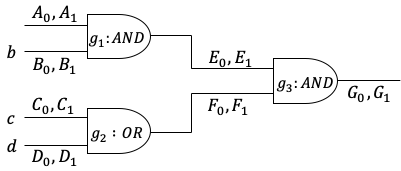
\includegraphics[scale = 0.6]{mid-circuit.png}
        \caption{The circuit and the garbled labels on each wire.}
        \label{fig:insert}
\end{figure}
    
    Let $\widehat{g}_1, \widehat{g}_2, \widehat{g}_3$ be the garbled gates of $g_1,g_2$ and $g_3$, respectively. The input labels are plotted in the figure. In this problem, we assume that all labels are of length $n$. Now suppose that an adversary Charlie learns the circuit, the garbled gates $\hat{g}_1$, $\hat{g}_2$ and $\hat{g}_3$, output wire labels $G_0,G_1$, as well as input wire labels $A_0, A_1, B_b, C_c, D_d$, where $b,c,d\in\{0,1\}$ are the inputs to the input wire labeled $B,C$ and $D$, respectively. Show how Charlie can use this information to learn at least one input out of $b$, $c$, or $d$ with probability $1-\sf{negl}(n)$ for some negligible function ${\sf negl}$. (Hint: How should the output of an AND gate change when you change one of the inputs? What does this tell you about the other input?)
\end{problem}
\begin{problemproof}
    Define an attack on $b$ s.t.

    Use the pair $(A_0,B_b)$ to decrypt $g_1$. Call the output $Y_0$.
    Use the pair $(A_1,B_b)$ to do the same. Call the output $Y_1$.

    If $Y_0 = Y_1$ then guess $b=0$.
    If $Y_0 \neq Y_1$ then guess $b=1$.

    probability:

    If $b=0$ then $(A_0,B_0)$ and $(A_1,B_0)$ will both decrypt to $E_0$ since $g_1$ is an and gate.

    If $b=1$ then $(A_0,B_1)$ and $(A_1,B_1)$ will decrypt to $E_0$ and $E_1$ respectively. Thus, these will only be equal with probability $2^{-n}$.

    Thus, $\P[B=b] \geq 1-2^{-n}$. Therefore, Charlie learns Bob's input with non-negligible probability.
\end{problemproof}

\begin{problem}{}
    Suppose you are given two commitment schemes $(\mathsf{com}_1, \mathsf{open}_1)$ and $(\mathsf{com}_2, \mathsf{open}_2)$ with the same message space and commitment space.
\end{problem}
\begin{subproblem}{}
    Suppose that both commitment schemes satisfy the perfectly binding property. However only one of them satisfies the computationally hiding property (but you don't
know which one). Construct a commitment scheme $(\mathrm{com}, \mathrm{open})$ which is both perfectly
binding and computationally hiding using only the provided commitment schemes
\end{subproblem}
\begin{problemproof}
    Assume we commit strings of length $n$.

    Define $(\mathrm{com}, \mathrm{open})$ s.t.

    For commit algorithm $\mathrm{com}(m,r)$ s.t. $r \in \{0,1\}^{2n}$. Let $r=r_1||r_2$.

    Compute $m_2 = \mathrm{com}_2(m,r_2)$

    Output $c=(\mathrm{com}_1(m_2,r_2))$
    
    \phantom{text}

    For open algorithm $\mathrm{open}(c,m,r=r_1||r_2)$
    
    Compute $m_2 =\com_2(m,r_2)$
    
    Compute $\mathrm{open}_1(c,m_2,r_1)$.

    If this rejects then reject.

    Return accept if it gets to here.

    \phantom{text}

    This is valid since if the committer followed the algorithm honestly then $\mathrm{open}(c,m,r=r_1||r_2)$ will accept if and only if $\mathrm{open}_1(c,\com_2(m,r_2),r_1)$ accepts, but since we assume both $\com_1$  and $\com_2$ are correct. This implies our combined algorithm is correct.

    Perfect Binding:

    Let $m_0,m_1 \in \bit^n$ and $r_0=r_{0,1}||r_{0,2},r_1=r_{1,1}||r_{1,2} \in \bit^{2n}$ s.t. $m_0 \neq m_1$

    Since $\com_2$ is perfectly binding then $m_2=\com_2(m_0,r_{0,2}) \neq \com_2(m_1,r_{1,2})=m_2'$. Then since $\com_1$ is perfectly binding this implies $\com_1(m_2,r_{0,1}) \neq \com_2(m_2',r_{1,1})$.

    Thus, the combined algorithm is perfectly binding.

    Computationally hiding:

    Let $m_0,m_1 \in \bit^n$. 

    Case 1: $(\mathrm{com}_1,\mathrm{open}_1)$ is computationally hiding.

    Assume there exists an adversary $D$ that could distinguish $\mathrm{com}(m_0,r)$ from $\mathrm{m_1,r}$ with non-negligible probability.

    Define $C$ on $\mathrm{com}_1$'s interface s.t.

    First run $D$ it will send us $m_0,m_1$.

    Then uniformly sample $s \in \bit^n$. Then compute $m_0'=\com_2(m_0,s), m_1'=\com_2(m_1,s)$ and then send $m,m'$ to the challenger.

    The challenger will then send back $\com_1(m_b',r)$.

    Then output $D$'s output.

    Since we simulate $\com$'s interface for $D$ this implies that $D$ will with non-negligible probability distinguish between $m_0$ and $m_1$ which implies $C$ will also distinguish with non-negligible probability.
    
    Case 2: $(\mathrm{com}_2,\mathrm{open}_2)$ is computationally hiding.

    Assume there exists an adversary $D$ that could distinguish $\mathrm{com}(m_0,r)$ from $\mathrm{m_1,r}$ with non-negligible probability.

    Define $C$ on $\mathrm{com}_2$'s interface s.t. 
    
    First run $D$ it will send us $m_0,m_1$.

    Then send $(m_0, m_1)$ to the challenger. Then uniformly sample $s \in \bit^n$.

    It will then send back $c_b = \mathrm{com}_2(m_b,r)$. Then compute $\com_1(m_b,s)$ and send this to $D$.

    Then output $D$'s guess.

    Since we simulate $\com$'s interface for $D$ this implies that $D$ will with non-negligible probability distinguish between $m_0$ and $m_1$ which implies $C$ will also distinguish with non-negligible probability.

    Therefore, in both cases it is computationally hiding.
\end{problemproof}

\begin{subproblem}{}
    Now suppose that both the commitments satisfy the computationally hiding property.
However, only one of them satisfies the perfectly binding property (but you don't know
which one). Construct a commitment scheme $(\mathrm{com}, \mathrm{open})$ which is both perfectly
binding and computationally hiding using only the provided commitment schemes.
\end{subproblem}
\begin{problemproof}
    Assume we commit strings of length $n$.

    Define $(\mathrm{com}, \mathrm{open})$ s.t.

    For commit algorithm $\mathrm{com}(m,r=r_1||r_2)$ s.t. $r \in \bit^{2n}$

    Let $c_1 \leftarrow \mathrm{com}_1(m,r_1)$ and $c_2 \leftarrow \mathrm{com}_2(m,r_2)$.

    Output $c=(c_1,c_2)$
    
    \phantom{text}

    For open algorithm $\mathrm{open}(c,m,r=r_1||r_2)$ s.t. $c=(c_1,c_2)$.

    Compute $\mathrm{open}_1(c_1,m,r_1)$.

    If this rejects then reject.

    Compute $\mathrm{open}_2(c_2,m,r_2)$
    
    If this rejects then reject.

    Return accept if it gets to here.

    This is valid since if the committer followed the algorithm honestly then $\mathrm{open}(c,m,r)$ will accept if and only if $\mathrm{open}_1(c,m,r_1)$ and $\mathrm{open}_2(c,m,r_2)$ accept, and since we assume that those are valid schemes this implies our combined scheme is also valid.

    Computationally hiding:
    
    Let $m_0 \neq m_1$

    Define hybrids $H_0,H_1,H_2$

    $H_0 = \{(\com_1(m_0,r_1)), \com_2(m_0,r_2) \mid r=r_1||r_2 \from U_{2n}\}$

    $H_1 = \{(\com_1(m_1,r_1)), \com_2(m_0,r_2) \mid r=r_1||r_2 \from U_{2n}\}$

    $H_2 = \{(\com_1(m_1,r_1)), \com_2(m_1,r_2) \mid r=r_1||r_2 \from U_{2n}\}$

    $H_0 \approx H_1$ since we know that $\com_1$ is computationally hiding, and $H_1 \approx H_2$ since we know that $\com_2$ is computationally hiding.

    Therefore, $\com$ is computationally hiding.

    Perfectly Binding:

    Case 1: $\com_1$ is perfectly binding.

    This implies that for $m_0 \neq m_1$ and for all $r_0=r_{0,1}||r_{0,2},r_1=r_{1,1}||r_{1,2} \in \bit^{2n}$ that 
    
    $(\com_1(m_0,r_{0,1}), \com_2(m_0,r_{0,2})) \neq (\com_1(m_1,r_{1,1}), \com_2(m_1,r_{1,2}))$ since $\com_1(m_0,r_{0,1}) \neq \com_1(m_1,r_{1,1})$.

    Case 2: $\com_2$ is perfectly binding.

    This is the same proof as above.

    Therefore, $\com$ is perfectly binding.
\end{problemproof}

\begin{problem}{}
    Consider two graphs $G_0 = (V_0,E_0) $ and $G_1= (V_1,E_1)$ where $V_b$ and $E_b$ are the vertices and edges respectively for graph $G_b$. We say the graphs are isomorphic if they are structurally the same. Formally, $G_0$ and $G_1$ are isomorphic if there exists a bijective function $\varphi: V_0 \to V_1$ such that for any two vertices $u,v \in V_0$, $(u,v) \in E_0$ if and only if $(\varphi(u),\varphi(v)) \in E_1$. Such a function $\varphi$ is called an isomorphism.
Paxton wants to prove to Valerie that $G_0$ is isomorphic to $G_1$ (denoted $G_0 \simeq G_1$),
but does not want to reveal any information about $\varphi$.
Consider the following protocol.
\vspace{1em}
\begin{mdframed}
    \vspace{0.5em}
    \textbf{Zero-Knowledge Proof for Graph Isomorphism}\\\\
    Initially, Paxton takes as input statement $(G_0, G_1)$ and witness $\varphi$. Valerie takes as input statement $(G_0, G_1)$.
    Paxton and Valerie repeat the following interaction for $n$ rounds where $n$ is the security parameter.
    \begin{enumerate}
        \item Paxton picks a random permutation $\pi$, computes graph $H = \pi(G_1)$, and sends $H$ to Valerie. Here, $\pi(G_1)$ essentially relabels the vertices of the graph based on the permutation.
        \item Valerie responds with a challenge $c\ \sample\ \{0, 1\}$.
        \item If $c = 0$, Paxton sends $\rho = \pi \circ \varphi$, and Valerie checks if $H = \rho(G_0)$. Here $\circ$ denotes functional composition (i.e. $\rho(G)$ first computes $G' = \varphi(G)$ then computes $\pi(G')$)
        \item If $c = 1$, Paxton sends $\rho = \pi$, and Valerie checks if $H = \rho(G_1)$.
    \end{enumerate}
\end{mdframed}
\vspace{1em}
\end{problem}

\begin{subproblem}{}
    Suppose that $G_0$ is not isomorphic to $G_1$. 
Show that for any possibly malicious prover, the probability 
that 
Valerie rejects in a \emph{single} fixed round is at least $\frac12$. 
\end{subproblem}
\begin{problemproof}
    Assume $G_0$ is not isomorphic to $G_1$.

    Let $H$ be an arbitrary graph.

    Assume for contradiction that the prover can successfully answer both challenges.

    This implies there exists $\rho_0,\rho_1$ s.t. $\rho_0(G_0)=H=\rho_1(G_1)$

    Rewriting we get that $G_1 = \rho_1^{-1} \circ \rho_0(G_0)$, but this implies that $G_0$ and $G_1$ are isomorphic which is a contradiction.

    Thus, $H$ is isomorphic to at most one. 
    
    Thus, $\P[H \cong G_0] \leq 1/2$.

    This implies the probability that Valerie rejects in a single fixed round is at least 1/2.
\end{problemproof}

\begin{subproblem}{}
    Suppose that $G_0$ is not isomorphic to $G_1$, and the prover 
can be arbitrarily malicious.
Please provide a lower bound on the probability that Valerie rejects in at least
one out of $n$ rounds. Give the tightest 
lower bound you can show, and justify your answer.
\end{subproblem}
\begin{problemproof}
    Given part (a) we know Valeria rejecting once is at least 1/2 probability. Thus, this implies that $\P[Valerie accepts] \geq 1/2$.

    Therefore, $\P[\t{Valeria rejects at least one round}] = 1 - \P[\t{Valeria accepts all rounds}]$.

    Since $\P[\t{Valerie accepts one round}] \geq 1/2 \implies \P[\t{Valerie accepts all rounds}] \geq 1/2^n$.

    Therefore, $\P[\t{Valeria rejects at least one round}] = 1 - \P[\t{Valeria accepts all rounds}] \geq 1-1/2^{n}$
\end{problemproof}

\begin{subproblem}{}
    Prove that the above construction is honest-verifier zero-knowledge. 
Intuitively, 
you want to show that the transcript the verifier sees by interacting with an honest prover is indistinguishable from a simulated transcript generated without knowledge of the witness.
We can capture this intuition by showing there exists a simulator that can spoof an accepting proof for a valid statement, even without the corresponding witness, so long as it sees the verifier's randomness ahead of time.

Formally, if indeed $G_0 \simeq G_1$, there must exist a PPT simulator $\mathcal{S}$ that on input $(G_0, G_1)$ can produce a message transcript $(H', c', \rho')$ indistinguishable from one generated by Paxton and Valerie. You may assume that Valerie always behaves honestly.
Please construct such a simulator. 
Show that your simulator is PPT, and informally argue why it produces a transcript indistinguishable from one generated by Paxton and Valerie.
\end{subproblem}
\begin{problemproof}
    Define $\mathcal{S}$ a simulator on $(G_0,G_1)$ and challenge bit $c' \in \{0,1\}$.

    1. Sample a random permutation $\sigma$ of the vertex set.
    2. If $c'=0$
        Set $H'=\sigma(G_0)$.
        Set $\rho=\sigma$.
    3. If $c'=1$
        Set $H'=\sigma(G_1)$.
        Set $\rho=\sigma$.
    4. Output $(H',c',\rho')$

    This is PPT since we can sample a permutation in $O(n)$.
    Computing $\sigma(G_{c'})$ can be done in polynomial time.

    This is indistinguishable since conditioned on the challenge bit $c$.
    
    If $c=1$:
        Real World: choose $\pi$ uniform, set $H=\pi(G_1), \rho=\pi, \t{output} (H,1,\rho)$
        Simulated: This does the same thing.
    If $c=0$:
        Same type of argument.
        
    Since $\pi$ and $\sigma$ are both uniform this implies that $(H,c,\pi)$ is identical to $(H,c,\sigma)$.
\end{problemproof}
\end{document}
